\documentclass[conference]{IEEEtran}
\IEEEoverridecommandlockouts
% The preceding line is only needed to identify funding in the first footnote. If that is unneeded, please comment it out.
%Template version as of 6/27/2024

\usepackage{cite}
\usepackage{amsmath,amssymb,amsfonts}
\usepackage{algorithmic}
\usepackage{graphicx}
\usepackage{textcomp}
\usepackage{xcolor}
\usepackage{url}
\usepackage{enumitem}
\usepackage{subcaption}
\def\BibTeX{{\rm B\kern-.05em{\sc i\kern-.025em b}\kern-.08em
    T\kern-.1667em\lower.7ex\hbox{E}\kern-.125emX}}

\newcommand{\groupcap}{\texttt{group\_cap}}
\newcommand{\groupcapreq}{\texttt{group\_cap\_req}}
\newcommand{\groupupdate}{\texttt{group\_update}}
\newcommand{\groupreq}{\texttt{group\_req}}
\newcommand{\channelupdate}{\texttt{channel\_update}}
\newcommand{\groupsize}{\texttt{group\_size}}
\newcommand{\mincaplimit}{\texttt{min\_cap\_limit}}
\newcommand{\maxcaplimit}{\texttt{max\_cap\_limit}}

\begin{document}

\title{Routing Method for Balancing Payment Privacy and Low Latency in Blockchain Payment Channel Networks}

\author{\IEEEauthorblockN{Kohei Sato}
	\IEEEauthorblockA{\textit{Graduate School of Engineering and Science} \\
		\textit{Shibaura Institute of Technology}\\
		Tokyo, Japan \\
		af20023@shibaura-it.ac.jp}
	\and
	\IEEEauthorblockN{Hiroaki Morino}
	\IEEEauthorblockA{\textit{Graduate School of Engineering and Science} \\
		\textit{Shibaura Institute of Technology}\\
		Tokyo, Japan \\
		morino@shibaura-it.ac.jp}
}

\maketitle

\begin{abstract}
	We propose the Group Capacity Broadcast (GCB) method that discloses only the minimum capacity among grouped payment channels, thereby reducing payment retries while preserving privacy. Simulation results on a real Lightning Network snapshot show that GCB shortens payment confirmation delay compared with the conventional method without sacrificing success rate.
\end{abstract}

\begin{IEEEkeywords}
	Blockchain, Payment Channel Network, Routing Method, Gossip Protocol
\end{IEEEkeywords}

\section{Introduction}

Payment channels (PCs) move most transactions off-chain and thus scale blockchains~\cite{poon_dryja_2016}. A Payment Channel Network (PCN) forwards a payment through several PCs, but the sender must choose a path whose every link has enough capacity (i.e., upstream balance).

Here a dilemma arises.  If each link publicly reveals its current balance, the sender can pick a feasible path on the first try, but privacy is lost because observers can trace payments.  If balances remain secret, privacy is kept, yet the sender learns feasibility only after the attempt, causing expensive retries and long delays.  Lightning's probabilistic routing slightly mitigates the delay but still struggles with large amounts.

This paper tackles the privacy–latency dilemma.  We evaluate the Group Capacity Broadcast (GCB) method, which discloses only the minimum balance inside a link group, thereby hiding individual balances while allowing the sender to rule out hopeless paths in advance.

\section{GCB Method}

GCB groups links with similar capacities and broadcasts only the minimum capacity within each group. A group constructor recruits links by broadcasting \groupreq{} messages specifying capacity range [\mincaplimit{}, \maxcaplimit{}]. Once \groupsize{} links join, the group must securely calculate its minimum capacity without exposing individual link balances.

The key innovation lies in a privacy-preserving minimum value computation protocol. Each group member initiates a \groupcap{} message containing its actual capacity and a unique identifier, which circulates through the group in a ring topology. As the message traverses each node, the capacity value is updated only if the current node's capacity is smaller, ensuring the final result represents the true minimum. To prevent observers from correlating capacity changes with specific links, nodes randomly abstain from updating the message approximately half the time during circulation. When a node receives its own message identifier after completing the full circuit, it recognizes the validity of the minimum value and broadcasts it network-wide as a \groupupdate{} message. This distributed consensus mechanism ensures that no single node can determine which link actually holds the minimum capacity, thereby maintaining payment privacy. Figure~\ref{fig:group_cap_handover} illustrates the detailed message flow of this protocol.

For routing decisions, senders can now determine path feasibility before transmission since each link's true capacity exceeds the disclosed group capacity. As shown in Figure~\ref{fig:capacities_in_group}, while individual links may have varying capacities, only the group's minimum capacity is revealed to the network. Senders use group capacity for grouped links and channel capacity for ungrouped links, applying standard shortest-path algorithms~\cite{lnd,eclair,clightning}. After successful payments, affected groups recalculate their minimum capacity to reflect balance changes, maintaining accuracy while preserving anonymity.

Privacy is preserved because observers cannot determine which specific link caused a group capacity change. Groups close when capacity updates exceed the initial range, triggering reformation with updated parameters to adapt to changing network conditions.

\begin{figure}[htbp]
	\centerline{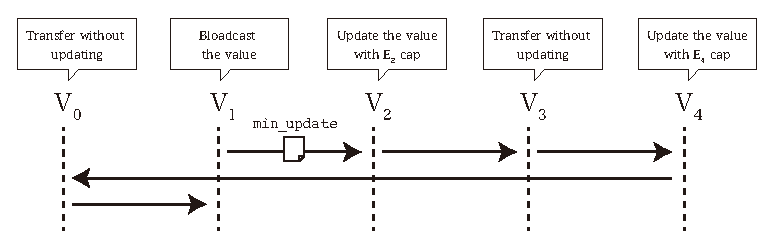
\includegraphics[width=\linewidth]{fig/group_cap_handover}}
	\caption{Group Capacity Calculation Protocol Message Flow}
	\label{fig:group_cap_handover}
\end{figure}

\begin{figure}[htbp]
	\centerline{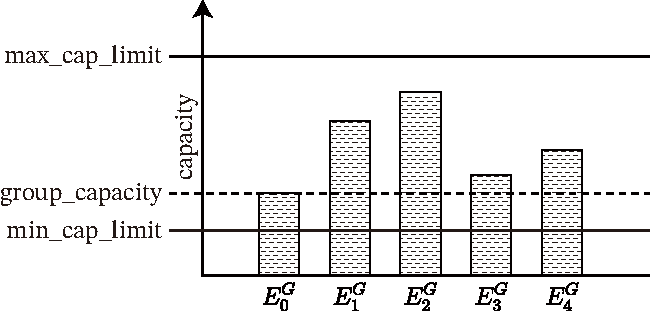
\includegraphics[width=0.85\linewidth]{fig/capacities_in_group}}
	\caption{Example of Capacity of Links Belonging to a Group and the Group Capacity}
	\label{fig:capacities_in_group}
\end{figure}

\section{Performance Evaluation}

This section evaluates the latency performance of the proposed GCB method using simulation.

\subsection{Evaluation Method}

\subsubsection{Parameters}

Group construction parameters are:
\begin{itemize}
	\item \groupsize{}: Number of links in a group
	\item $\alpha$: Parameter determining group capacity conditions \mincaplimit{} and \maxcaplimit{} where $0 < \alpha < 1$
\end{itemize}

When the group constructor's initial link registered in the group is $E_{const}$ with capacity $cap(E_{const})$, group capacity conditions \mincaplimit{} and \maxcaplimit{} are set using parameter $\alpha (0 < \alpha < 1)$ as:
\begin{align}
	\mincaplimit & = cap(E_{const}) \times (1-\alpha) \\
	\maxcaplimit & = cap(E_{const}) \times (1+\alpha)
\end{align}

\subsubsection{Evaluation Metrics}

Main evaluation metrics are:
\begin{itemize}
	\item Success Rate: Ratio of successful payments to all attempted payments
	\item Latency (Success): Average delay time until successful payment confirmation [ms]
\end{itemize}

\subsubsection{Simulation Conditions}

We extended the payment channel network simulator CLoTH~\cite{CONOSCENTI2021100717}, which accurately reproduces Lightning Network HTLCs, implementing the GCB method along with two comparison methods:
\begin{itemize}
	\item LN method: Lightning Network method using \channelupdate{} for probabilistic payment route determination
	\item RBB method: Real-time Balance Broadcast (complete disclosure of all link capacities without privacy consideration)
\end{itemize}

We used a Lightning Network snapshot from December 17, 2020, with 6005 nodes and 60913 links. This data was obtained from LND's \texttt{describegraph} command, containing all publicly available information identical to the actual network. Since initial PC balances are undisclosed, we set them using uniformly distributed random numbers. We performed 5000 payments with amounts following normal distribution (mean $\mu = 10000$ sats, variance $\sigma = \mu \times 0.1$) and uniformly distributed random sender/recipient selection.

\subsection{Latency Evaluation}

Using optimal parameters $\groupsize=10, \alpha=0.1$, we compared GCB and LN methods for varying average payment amounts. Results show that while LN method confirmation delays increase significantly with payment amount, GCB method delays increase relatively little. For large payments, LN method experiences many retries due to considering only failure frequency without link capacity, prolonging confirmation time. GCB method eliminates unnecessary retries by disclosing group capacity, enabling immediate pre-send determination of impossible payments and minimizing confirmation delay increases even for large amounts, as demonstrated in Fig.~\ref{fig:pmt_amt_vs_time}.

\begin{figure}[htbp]
	\centerline{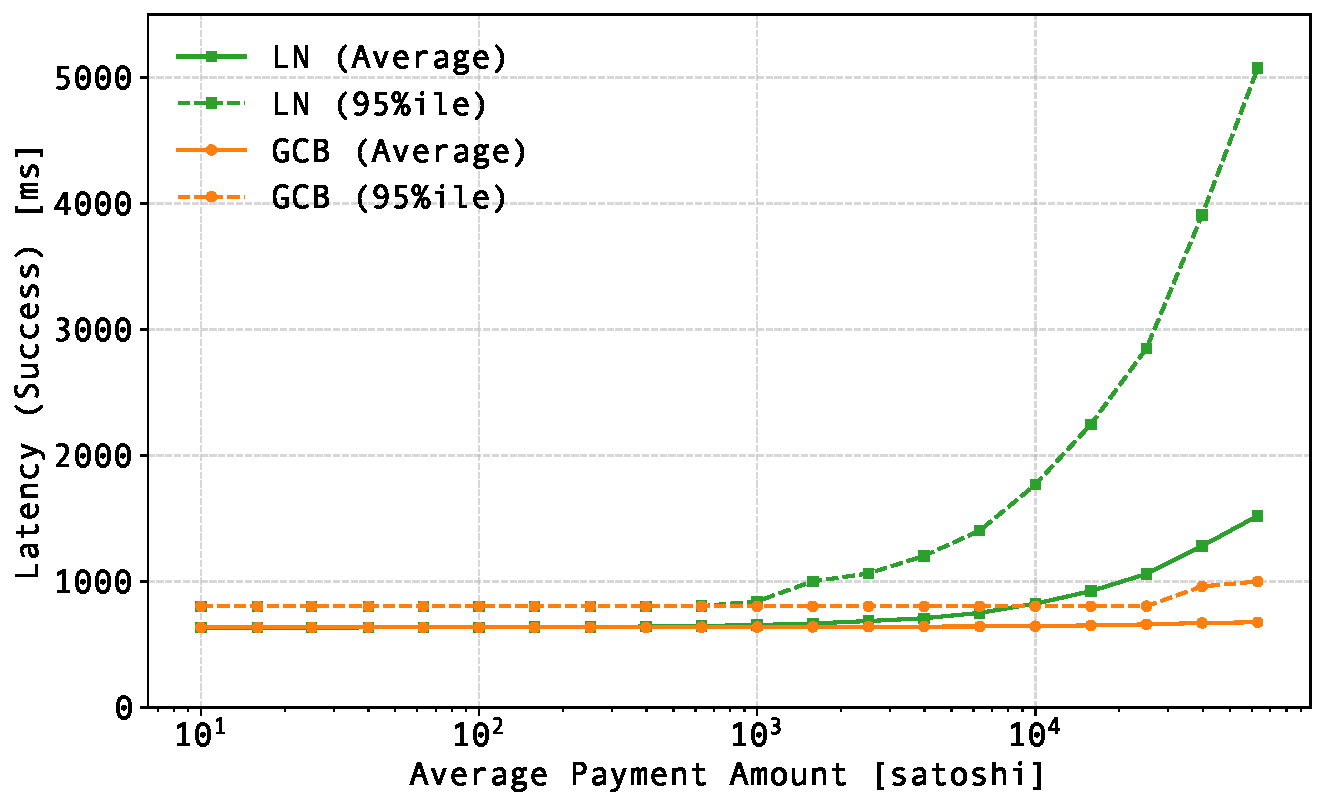
\includegraphics[width=\linewidth]{fig/pmt_amt_vs_time}}
	\caption{Latency of Sending Payment vs Payment Amount for Successful Cases Only}
	\label{fig:pmt_amt_vs_time}
\end{figure}

\section{Conclusion}

Simulation results confirmed that the proposed GCB method considerably shortens payment confirmation delay while maintaining a high success rate. Future work includes verifying payment information confidentiality under more diverse attack models.

\begin{thebibliography}{00}
	\bibitem{nakamoto2008bitcoin} S. Nakamoto, ``Bitcoin: A peer-to-peer electronic cash system,'' 2008.
	\bibitem{poon_dryja_2016} J. Poon and T. Dryja, ``The bitcoin lightning network: Scalable off-chain instant payments,'' 2016.
	\bibitem{lnbolt} ``BOLT: Basis of Lightning Technology,'' \url{https://github.com/lightningnetwork/lightning-rfc}.
	\bibitem{lnd} ``Lightning Network Daemon,'' \url{https://github.com/lightningnetwork/lnd}.
	\bibitem{clightning} ``Core Lightning,'' \url{https://github.com/ElementsProject/lightning}.
	\bibitem{eclair} ``Eclair,'' \url{https://github.com/ACINQ/eclair}.
	\bibitem{Andreescu_2021} O. Andreescu et al., ``Optimizing payment routing in the lightning network,'' in Proc. IEEE INFOCOM, 2021.
	\bibitem{published_papers/48227240} K. Sato and H. Morino, ``Group capacity broadcast method for payment channel networks,'' Technical Report, 2023.
	\bibitem{CONOSCENTI2021100717} M. Conoscenti et al., ``CLoTH: A simulator for HTLC payment networks,'' Future Generation Computer Systems, vol. 118, pp. 1--17, 2021.
\end{thebibliography}

\end{document}
